\documentclass{article}
\usepackage{amsmath} % For more maths
\usepackage{graphicx} % For images
\usepackage{hyperref} % For link support (also turns figure refs to clickable links)
\usepackage{xcolor} % For coloured text
\usepackage[numbers]{natbib} % Sophisticated bibliography with commands for \citeauthor and \citetitle (`biblatex` is an alternative)

\bibliographystyle{plainnat} % We choose the "plain" reference style


\title{More \LaTeX{}}
\author{MU}
\date{2\textsuperscript{nd} May 2022}

\begin{document}
    \maketitle

    \section{Overview}
    This document shows you what is possible in \LaTeX{}, including some extra stuff that wasn't explicitly gone through in the workshop slides\footnote{Like this! This is a footnote!}.

    \begin{itemize}
        \item Footnotes
        \item Referring to equations and figures
        \item Underbraces and overbraces
        \item URLs and links
    \end{itemize}

    \section{Pythagoras}
    Pythagoras was an ancient Ionian Greek philosopher who lived around 570~BC. % The tilde here means that 570 BC will not flow onto separate lines!
    He is often credited with the Pythagorean theorem, listed below in equation \eqref{eq:pythag}, although there is evidence that the theorem was known about in ancient Egypt before Pythagoras.
    \begin{equation}
        \underbrace{a^2 + b^2}_\text{sides} = \overbrace{c^2}^\text{hypotenuse}
        \label{eq:pythag}
    \end{equation}

    Also, he may have had a cult\footnote{Check out this url (\url{https://en.wikipedia.org/wiki/Pythagoreanism}). Or check out \href{https://en.wikipedia.org/wiki/Pythagoreanism}{\color{blue}\underline{this interactive link}}(note the link by default has no style)}.


    \subsection{Proof of the Pythagorean theorem}
    We can prove the Pythagorean theorem. Looking at figure \ref{fig:pythag-image} we can see the setup, and figure \ref{fig:pythag-working} has the working.
    
    \begin{figure}
        \centering
        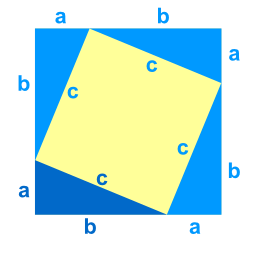
\includegraphics[width=0.5\textwidth]{img/pythag.png}
        \caption{Geometry setup}
        \label{fig:pythag-image}
    \end{figure}

    \begin{figure}
        \begin{align*}
            \text{Inner square area} &\rightarrow c^2\\
            \text{Triangle area} &\rightarrow \frac{ab}{2}\\
            \text{Area of larger square}\rightarrow(a+b)(a+b) &= c^2 + 2ab \leftarrow\text{Sum of shapes}\\
            a^2 + b^2 + 2ab &=  c^2 + 2ab\\
            a^2 + b^2 &=  c^2
        \end{align*}
        \caption{Proof}
        \label{fig:pythag-working}
    \end{figure}

    \section*{How to cite things}  % An un-numbered section
    Ok, so we need to cite some things. There are many texts that talk about Pythagoras\cite{Fauvel2009,Huffman2018,Joost2009}.

    \begin{itemize}
        \item \citeauthor{Fauvel2009} talks about...
        \item \citeauthor{Huffman2018} talks about...in
        \item \citeauthor{Joost2009} talks about...
    \end{itemize}
    
    \bibliography{refs} % Entries are in the refs.bib file

\end{document}